\documentclass{article}

\title{Comparing CART and CTree: A simulation study}

\usepackage{Sweave}
\begin{document}
\Sconcordance{concordance:code_for_tables.tex:code_for_tables.Rnw:%
1 4 1 1 0 4 1 1 45 1 13 16 0 1 2 1 37 1 11 16 0 1 2 1 44 1 11 16 0 1 2 %
1 1 1 48 1 10 15 0 1 2 1 321 1 1 1 81 1 2 1 1}


\maketitle


% latex table generated in R 3.4.0 by xtable 1.8-2 package
% Sat Aug 12 20:29:20 2017
\begin{table}[ht]
\centering
\begin{tabular}{rlllll}
  \hline
 & MSE &  & Terminal Node &  &  \\ 
  \hline
 & Mean & SD & Mean & 20th & 80th \\ 
  CART & 4.12 & 0.413 & 15 & 14 & 16 \\ 
  Pruned CART & 4.19 & 0.442 & 14 & 13 & 16 \\ 
  Pruned CART (1-SE) & 4.55 & 0.509 & 9 & 6 & 11 \\ 
  CTree & 4.14 & 0.409 & 14 & 13 & 15 \\ 
  Linear Regression & 1.03 & 0.093 &  &  &  \\ 
   \hline
\end{tabular}
\caption{Regression model} 
\end{table}

% latex table generated in R 3.4.0 by xtable 1.8-2 package
% Sat Aug 12 20:29:21 2017
\begin{table}[ht]
\centering
\begin{tabular}{rlllll}
  \hline
 & MSE &  & Terminal Node &  &  \\ 
  \hline
 & Mean & SD & Mean & 20th & 80th \\ 
  CART & 1.26 & 0.151 & 7 & 6 & 8 \\ 
  Pruned CART & 1.22 & 0.137 & 4 & 3 & 5 \\ 
  Pruned CART (1-SE) & 1.25 & 0.139 & 3 & 3 & 4 \\ 
  CTree & 1.27 & 0.154 & 4 & 3 & 4 \\ 
  Linear Regression & 2.04 & 0.179 &  &  &  \\ 
   \hline
\end{tabular}
\caption{ Tree model} 
\end{table}

% latex table generated in R 3.4.0 by xtable 1.8-2 package
% Sat Aug 12 20:29:21 2017
\begin{table}[ht]
\centering
\begin{tabular}{rlllll}
  \hline
 & MSE &  & Terminal Node &  &  \\ 
  \hline
 & Mean & SD & Mean & 20th & 80th \\ 
  CART & 1.39 & 0.138 & 13 & 11 & 15 \\ 
  Pruned CART & 1.37 & 0.131 & 6 & 3 & 9 \\ 
  Pruned CART (1-SE) & 1.37 & 0.133 & 3 & 2 & 3 \\ 
  CTree & 1.34 & 0.126 & 5 & 4 & 6 \\ 
  Linear Regression & 1.17 & 0.106 &  &  &  \\ 
   \hline
\end{tabular}
\caption{Hybrid model} 
\end{table}


% latex table generated in R 3.4.0 by xtable 1.8-2 package
% Sat Aug 12 20:29:21 2017
\begin{table}[ht]
\centering
\begin{tabular}{rlll}
  \hline
 & Mean (MSE) & Mean (SD) & Type I Error (Mean) \\ 
  \hline
CART & 0.65 & 0.07 & 1 \\ 
  Pruned CART & 0.99 & 0.091 & 0.0559 \\ 
  Pruned CART (1-SE) & 1 & 0.089 & 3e-04 \\ 
  CTree & 0.99 & 0.089 & 0.0513 \\ 
  Linear Regression & 0.97 & 0.088 &  \\ 
   \hline
\end{tabular}
\caption{Type I error model} 
\end{table}

\section*{Figure 5}
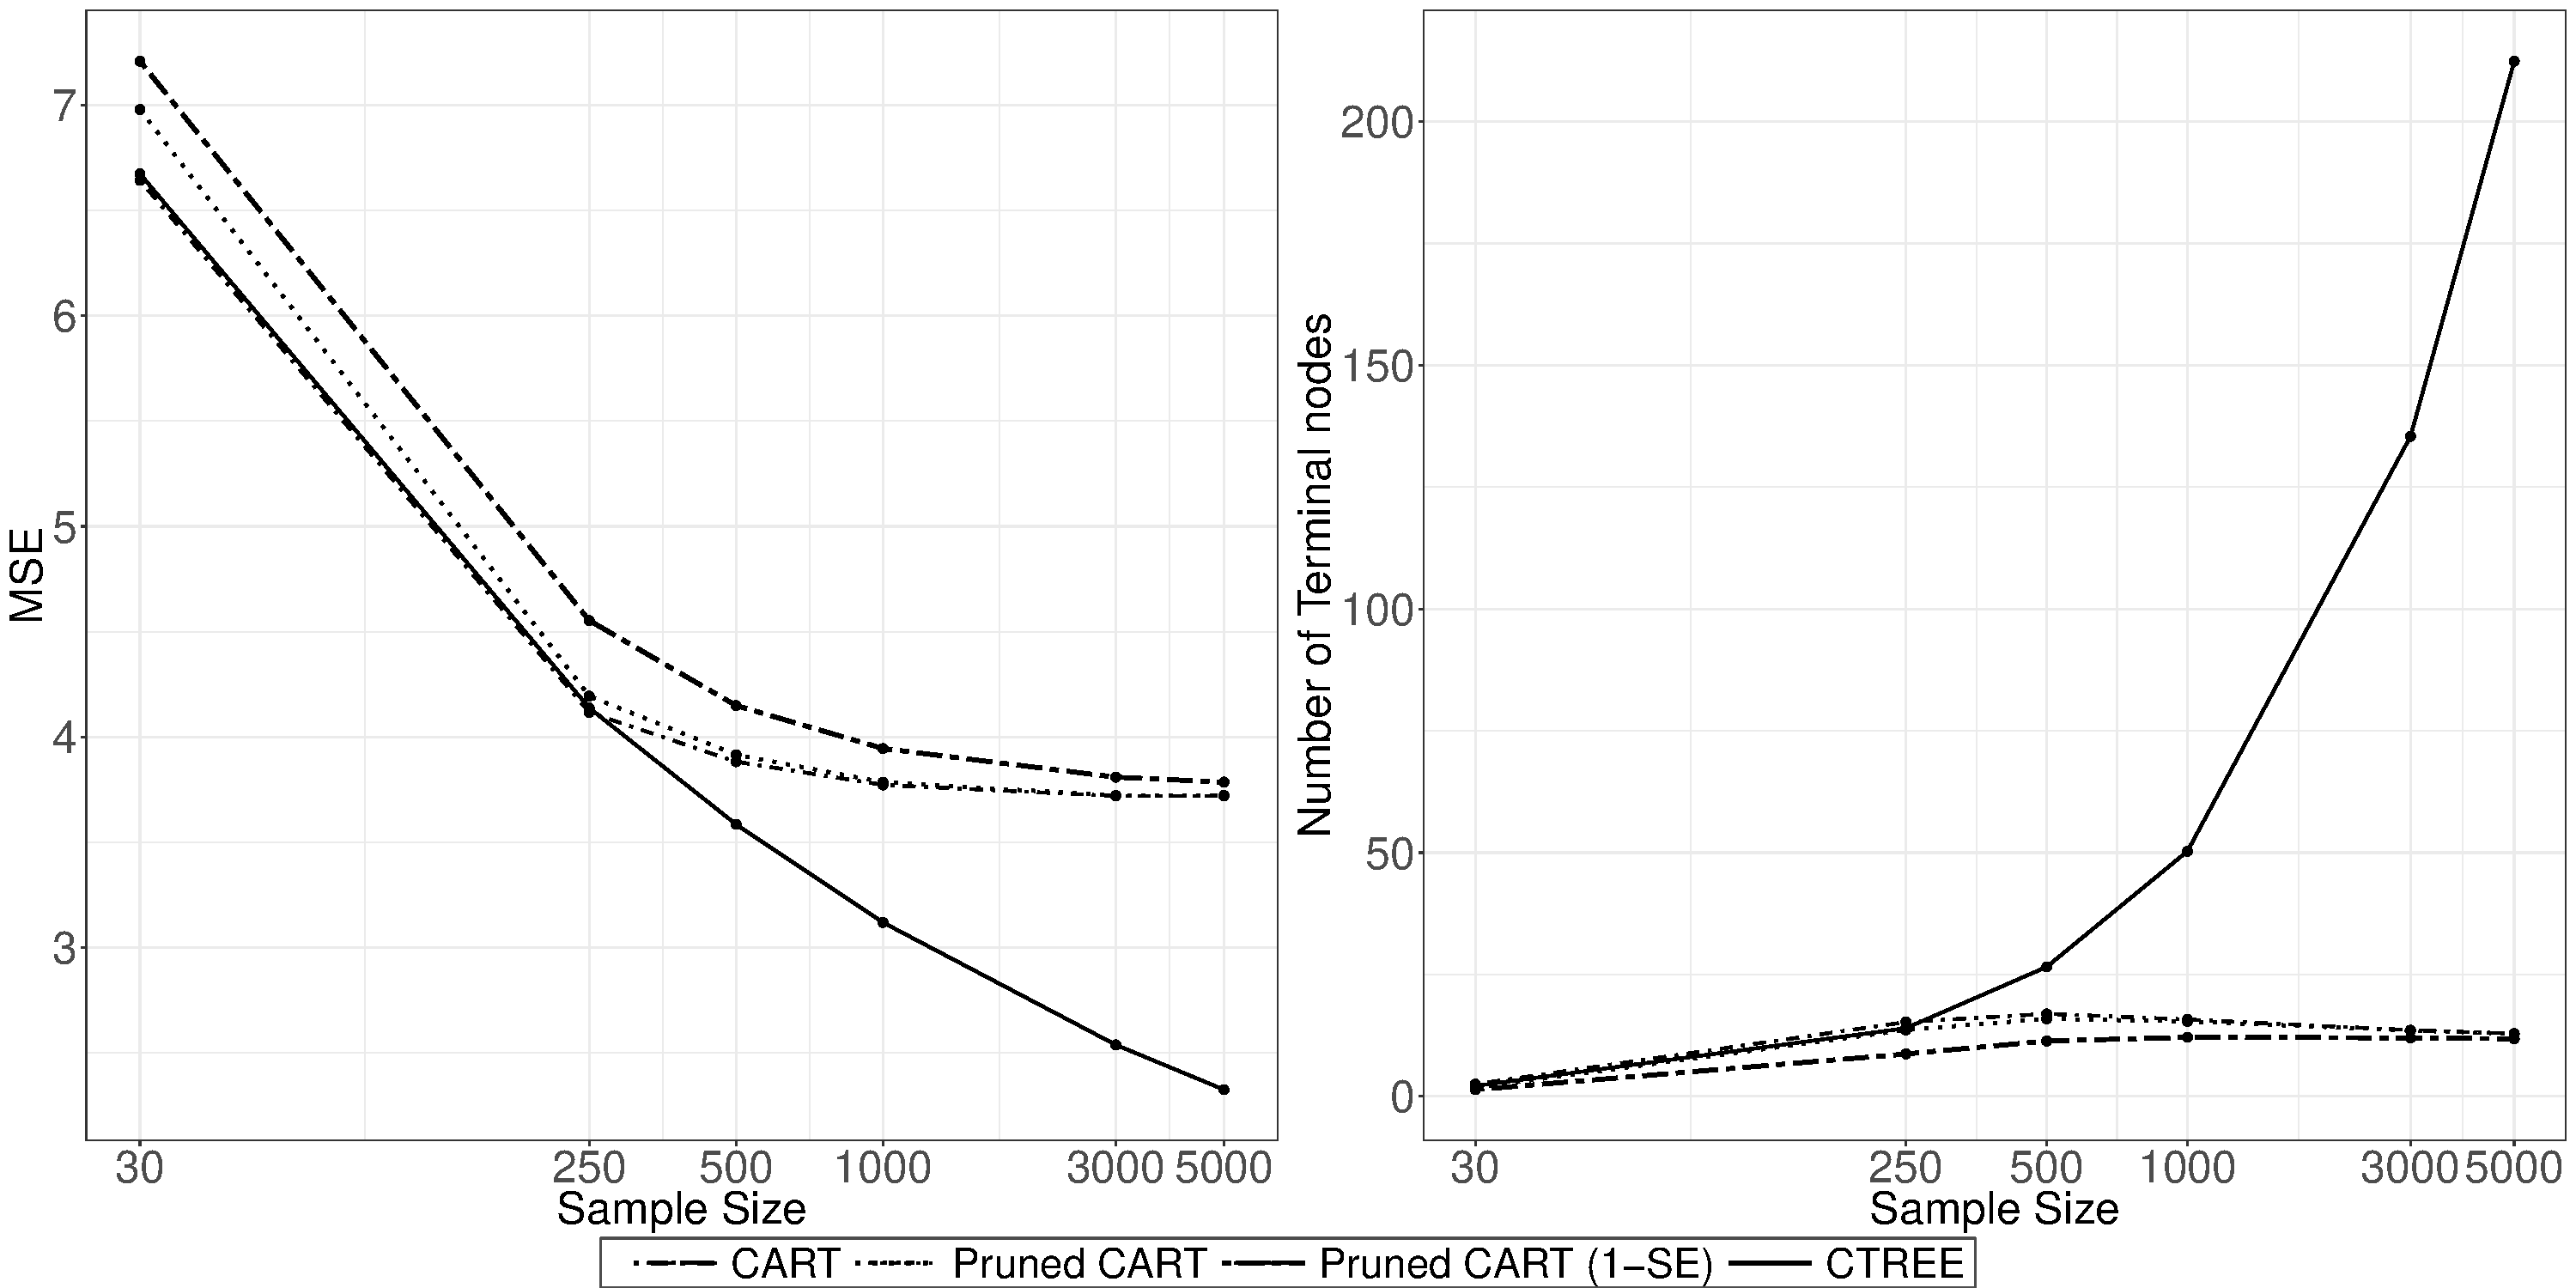
\includegraphics{code_for_tables-010}

\end{document}
